\newpage
\hypertarget{multiMOSL}{}
\subsection{Working with multple MOSL projects}
\texHeader

% Eclipse import instructions; all unconfirmed.
\begin{itemize}

\item[$\blacktriangleright$] Confirm your source metamodel \texttt{LeitnersLearningBox}, is in the current workspace prepared and right-click on
\texttt{MyWorkingSet}. Select \texttt{Import\ldots} from the context menu (Fig.~\ref{fig:eclipseContextImport}).

\vspace{0.25cm}

\begin{figure}[htbp]
\begin{center}
  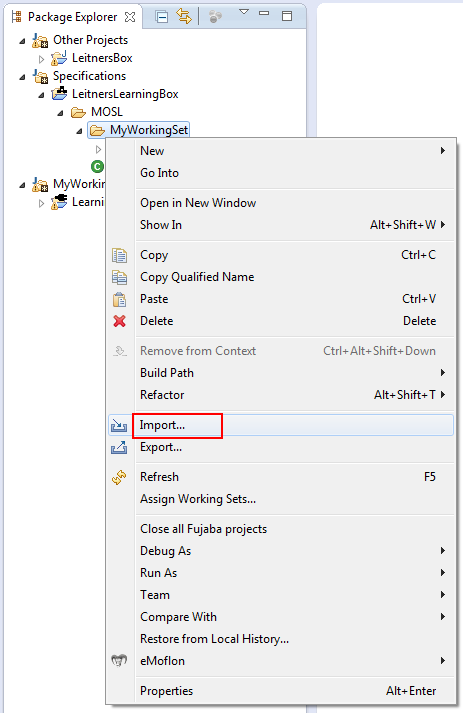
\includegraphics[width=0.6\textwidth]{eclipse_contextImport}
  \caption{Starting the import process in Eclipse}
  \label{fig:eclipseContextImport}
\end{center}
\end{figure}

\item[$\blacktriangleright$] In the first dialogue, set your import source by navigating to ``General/File System.'' This is the appropriate choice since
we want to import the entire directory structure of the target metamodel, not a pre existing project.

\item[$\blacktriangleright$] Press \texttt{Browse\ldots} and navigate to the folder where you extracted the contents of the \texttt{Part4.zip} download file
which included this document (Fig.~\ref{fig:importFileSys}). Press \texttt{Select All} to ensure you're importing all the necessary MOSL files for your TGG
target metamodel. Affirm and close the dialogue by pressing \texttt{Finish}.

\newpage

\begin{figure}[htbp]
\begin{center}
  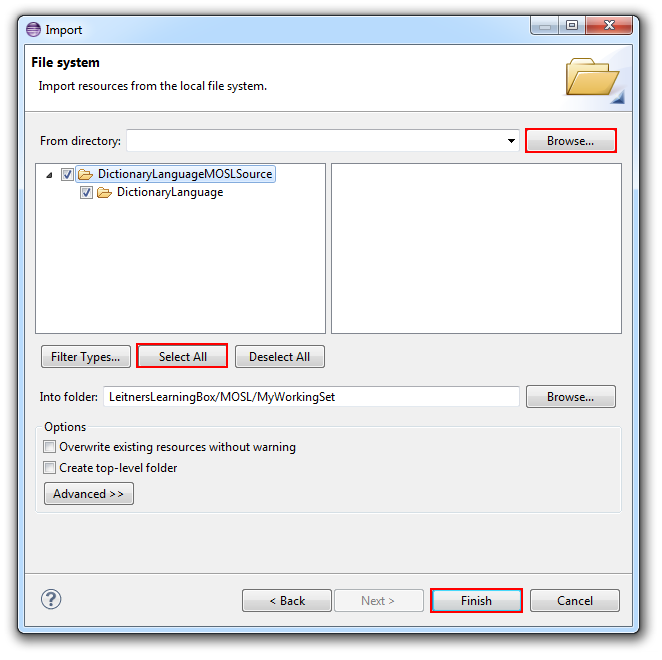
\includegraphics[width=0.8\textwidth]{eclipse_importDialogue}
  \caption{Importing the \texttt{target} metamodel into your workspace}
  \label{fig:importFileSys}
\end{center}
\end{figure}

\item[$\blacktriangleright$] With your project now loaded, navigate to ``Build (Without Cleaning)'' on the toolbar to build both metamodels. Confirm with
Fig.~\ref{fig:bothmetamodelstructures} that your MOSL directory is now populated with both metamodels, and notice that a second \texttt{Dictionary\-Language}
folder appeared under the same node as the \texttt{LearningBoxLanguage} repository project. If you expand this folder, you'll be able to see that it has
similar generated code for the imported metamodel.

\begin{figure}[htbp]
\begin{center}
  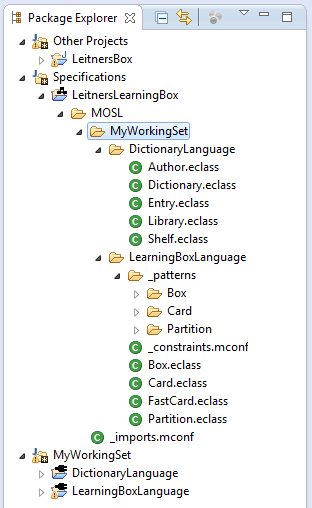
\includegraphics[width=0.5\textwidth]{eclipse_metamodelStructures}
  \caption{Fully loaded dual-metamodel structure}
  \label{fig:bothmetamodelstructures}
\end{center}
\end{figure}

\item[$\blacktriangleright$] Great work -- You're now ready to start using your metamodels in a TGG transformation! If you've just joined us and are interested
in the eMoflon project structure, or curious as to how Java code is generated, we invite you to read Section 4.2 from Part I. Otherwise, continue to the next section to begin
building your TGG Schema. 

\end{itemize}
